\documentclass[tikz,border=6pt]{standalone}
\usepackage{pgfplots}
\usepgfplotslibrary{groupplots}
\usetikzlibrary{calc}
\pgfplotsset{compat=1.18}
\begin{document}
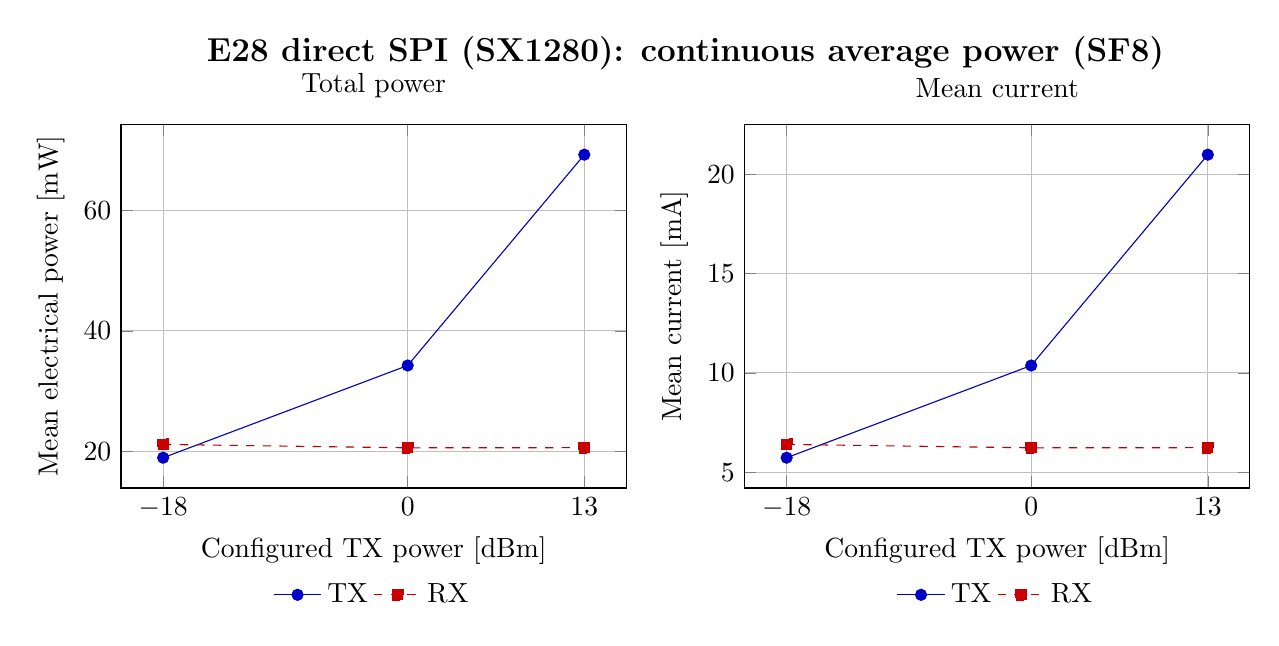
\begin{tikzpicture}
\begin{groupplot}[group style={group size=2 by 1,horizontal sep=1.5cm},width=8cm,height=6.2cm,xtick={-18,0,13},xlabel={Configured TX power [dBm]},grid=both,legend style={draw=none,at={(0.5,-0.23)},anchor=north,legend columns=2}]
\nextgroupplot[title={Total power},ylabel={Mean electrical power [mW]}]
\addplot+[blue!75!black,mark=*] coordinates {(-18,18.8984291) (0,34.2373864) (13,69.3064568)};\addlegendentry{TX}
\addplot+[red!75!black,dashed,mark=square*] coordinates {(-18,21.1124903) (0,20.5455339) (13,20.5686218)};\addlegendentry{RX}
\nextgroupplot[title={Mean current},ylabel={Mean current [mA]}]
\addplot+[blue!75!black,mark=*] coordinates {(-18,5.72679669) (0,10.3749656) (13,21.0019566)};\addlegendentry{TX}
\addplot+[red!75!black,dashed,mark=square*] coordinates {(-18,6.39772433) (0,6.22591936) (13,6.23291569)};\addlegendentry{RX}
\end{groupplot}
\node[font=\bfseries\large] at ($(group c1r1.north)!0.5!(group c2r1.north)+(0,0.9cm)$) {E28 direct SPI (SX1280): continuous average power (SF8)};
\end{tikzpicture}
\end{document}
